\section{Trajectory analysis} \label{ch:trajectory}

**intro**

\subsection{Governing equations}\label{sec:gov}

\begin{wrapfigure}{r}{0.4\textwidth}
		\centering
		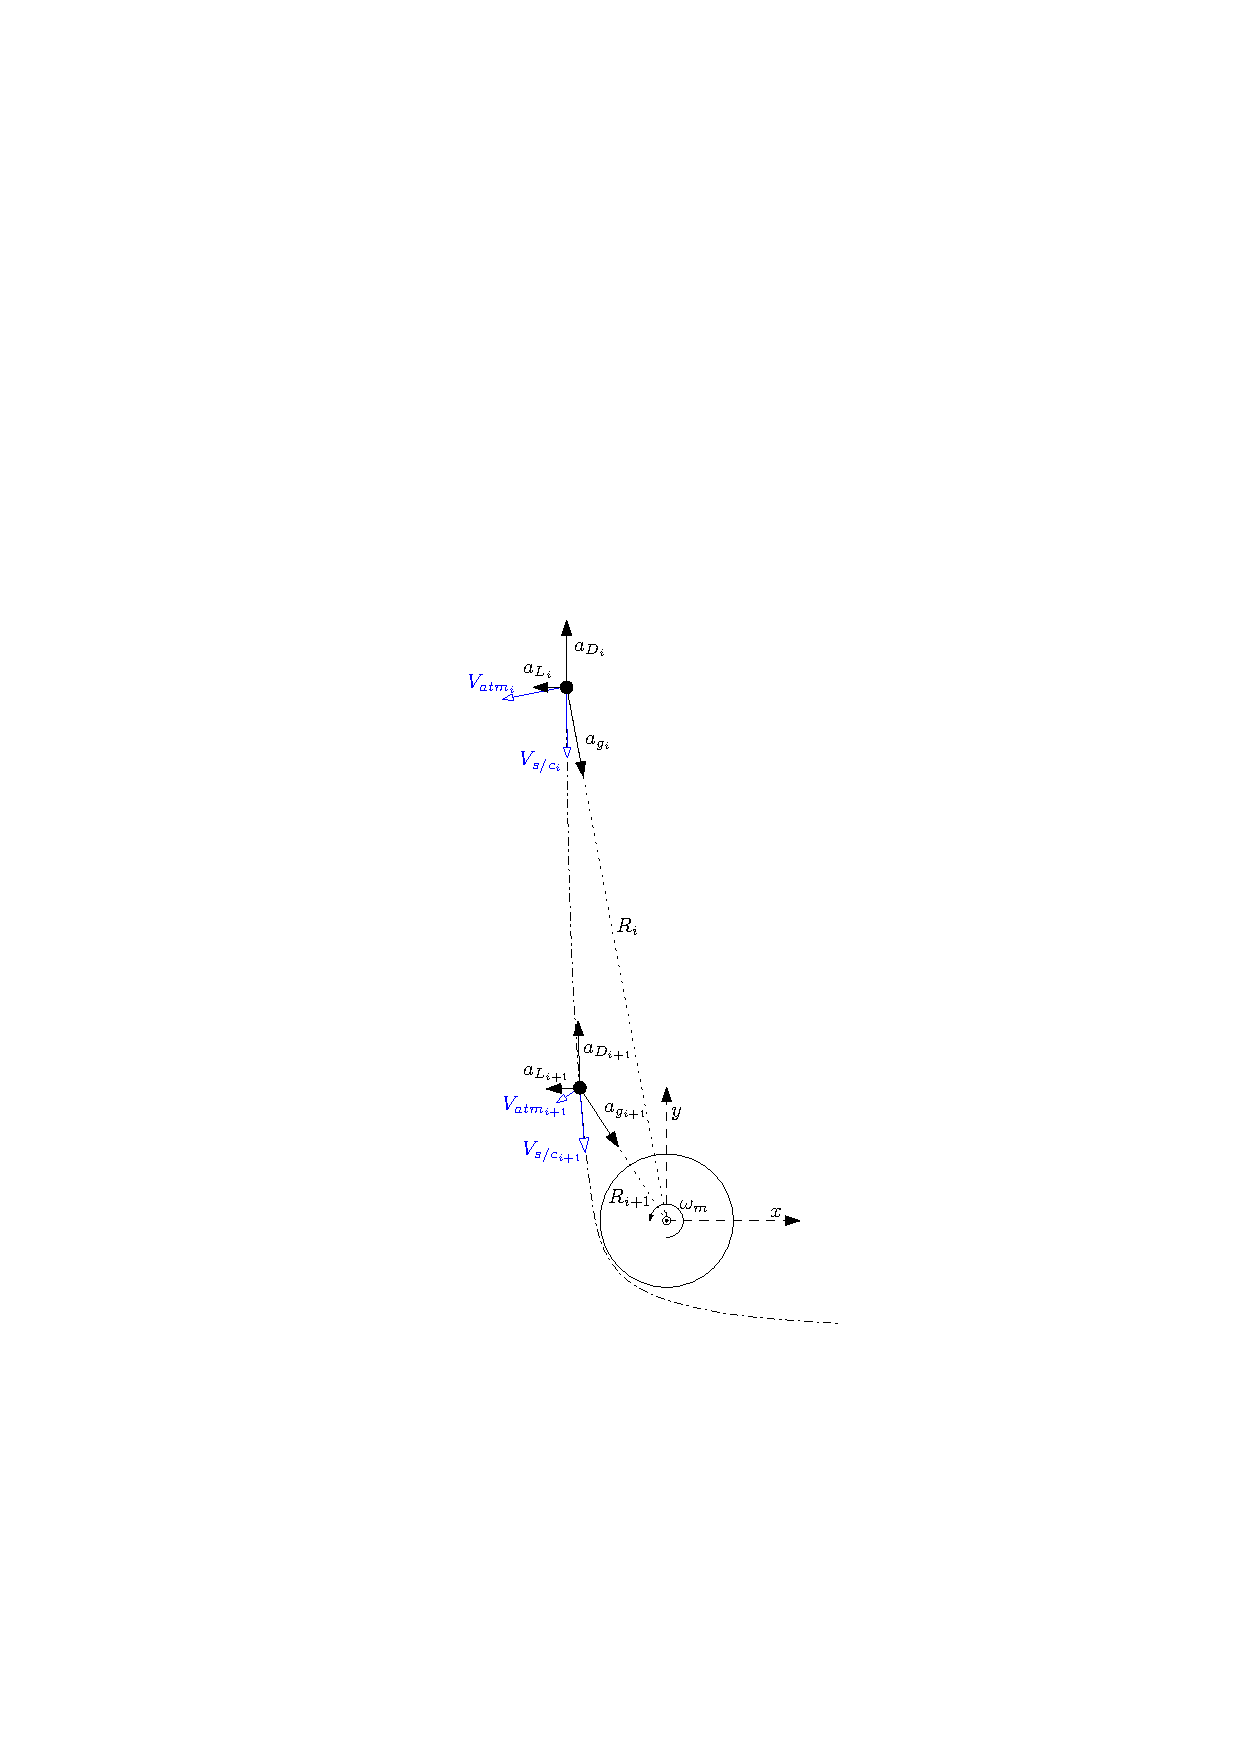
\includegraphics[width = 0.4\textwidth]{Figure/orbital_mechanics.pdf}
		\caption{The kinetic diagram visualizing the governing equations of the trajectory analysis}
		\label{fig:orb}
\end{wrapfigure}

The motion of a spacecraft can be broken down in some dominant contributors. These are the gravitational pull and the aerodynamic forces. Disturbances like solar radiation or gravitational pull from other bodies is neglected in the model.

To be able to fully describe the contributors, two reference frames need to be defined. The non rotating inertial frame is defined with its origin in the centre of mass of Mars (if it would be perfectly spherical), this is the \gls{mci}. 
Another reference frame is the \gls{mcmf}, in our first model the origin and the z-axis of both reference frames is equal (so no axis tilt is taken into account). The difference between the two is that the \gls{mcmf} is rotating around the z-axis with rotational velocity \gls{con:omegamars} compared to the \gls{mci}.

The gravitational pull is described by Newtons law of gravitation, together with Newton's second law, it can be written as an acceleration as in equation \ref{eq:nG}.

\begin{equation} \label{eq:nG}
\gls{sym:g} = -\frac{\gls{con:G}\gls{con:Mmars}}
					{\gls{sym:R}^3}\gls{sym:Rv}
\end{equation}

The aerodynamic forces are described by the lift and the drag, these forces are acting in the direction and orthogonal to the velocity of the spacecraft with respect to the atmosphere, this is the velocity of the spacecraft in the \gls{mcmf}. This velocity needs to be converted to \gls{mci} to be able to express the aerodynamic forces in the \gls{mci}, as in equation \ref{eq:Vsc_mcmf_mci}.

\begin{equation} \label{eq:Vsc_mcmf_mci}
\left.\gls{sym:Vvsc}\right|_{MCMF}^{MCI} = \gls{sym:Vvsc}_{,a} = \left.\gls{sym:Vvsc}\right|_{MCI} - \left(\gls{con:Omegamars} \times \gls{sym:Rv} \right)
\end{equation}

The aerodynamic accelerations due to the lift and the drag are described by equations \ref{eq:aL} and \ref{eq:aD} respectively.

\begin{equation} \label{eq:aL}
\gls{sym:aL} = \frac{\gls{sym:CL}\gls{sym:rho}\gls{sym:A}}{2 \gls{sym:m}} 
				\left|\gls{sym:Vvsc}_{,a}\right|^2
				\frac{\gls{sym:Vvsc}_{,a} \times \mathbf{z}}
				{\left| \gls{sym:Vvsc}_{,a} \times \mathbf{z}\right|}
\end{equation}

\begin{equation} \label{eq:aD}
\gls{sym:aD} = \frac{\gls{sym:CD}\gls{sym:rho}\gls{sym:A}}{2 \gls{sym:m}}
				\left|\gls{sym:Vvsc}_{,a}\right|^2 \frac{\gls{sym:Vvsc}_{,a}}{\left|\gls{sym:Vvsc}_{,a}\right|}
\end{equation}

The total acceleration is now the summation of the gravitational, lift and drag acceleration as in equation \ref{eq:aD}.

\begin{equation} \label{eq:acc}
\gls{sym:acc} = \gls{sym:g} + \gls{sym:aL} + \gls{sym:aD}
\end{equation}

If the acceleration is assumed to be constant for small time steps, then the new position and velocity can be determined by discretizing the dynamic equations of motion resulting in equations \ref{eq:ai} till \ref{eq:Ri}.

\begin{equation} \label{eq:ai}
\gls{sym:acc}_i = \gls{sym:g}_i + \gls{sym:aL}_i + \gls{sym:aD}_i
\end{equation}

\begin{equation} \label{eq:Vi}
\gls{sym:Vv}_{i+1} = \gls{sym:Vv}_i + \gls{sym:acc}_i \gls{sym:Dt}
\end{equation}

\begin{equation} \label{eq:Ri}
\gls{sym:Rv}_{i+1} = \gls{sym:Rv}_i + \gls{sym:Vv}_i \gls{sym:Dt} + \gls{sym:acc}_i \gls{sym:Dt}^2
\end{equation}

\subsection{Program structure}\label{sec:prog_struct}

In order to use the governing equations (equations \ref{eq:ai}, \ref{eq:Vi} and \ref{eq:Ri}) to produce usefull results they have to be implemented in a simulation which calculates the trajectory. From this calculated trajectory the program has to extract usefull data and conclusions. To model aerodynamic forces on the spacecraft an atmosphere model is needed. The atmosphere model used is presented in subsection \label{subsec:atmos}. The three different modules comprising the program are discribed in subsection \ref{subsec:modules}. In subsection \ref{subsec:flow} a flowchart of the program is presented.

\subsubsection{Atmosphere model}\label{subsec:atmos}
As stated in Section \ref{sec:control}, for the atmospheric model the NASA software \gls{marsgram} is used. The atmospheric properties are queried at equally spaced points: at all latitudes and longitudes at an interval of $10$ $[^\circ]$, and heights from $0$ to $400$ $[km]$ at an interval of $5$ $[km]$. The software generates data based on equations for atmosphere properties and incorporates the high amount of dust on Mars, which has a big effect on the absorbed radiation heat from the sun. The output of the program is, among others, the density, temperature and gas composition at that query point, along with other less important parameters. \cite{Justus2001}
This data is then saved for processing during trajectory simulation. In the trajectory simulation software, the atmospheric properties at certain points in the atmosphere are required. The discrete atmosphere data is thus interpolated to obtain an estimate of there properties. 

\subsubsection{Modules} \label{subsec:modules}

The program first implements the governing equations on each time step. Secondly three modules were created, two to find feasible orbits and another to calculate the full orbit of the orbits which are found to be feasible. These four modules are described below.

\paragraph{Implementation of governing equations}\textit{orbit.m}

The module implementing the governing equations has a lot of input data of which most are constants and design parameters. One of the inputs is the dataset created by the atmospheric model described in subsection \ref{subsec:atmos}. The density and gravitational acceleration taken from this dataset is different for each cycle of the program and dependent on the height, longitude and latitude of the spacecraft. Also the previous location, velocity and acceleration (in vector form) are constantly changing inputs.

The input variables are directly filled in into equations \ref{eq:ai}, \ref{eq:Vi} and \ref{eq:Ri}. This creates output values for the location, velocity and acceleration. Both the total acceleration and the separate accelerations due to the drag, lift and gravitation are outputted.

\paragraph{Orbit selection} \textit{orbit\_selection.m}

The module has a lot of constants, initial conditions and design parameters as input variables. One of the input variables is the starting distance in y-direction (using the reference frame from figure \ref{fig:orb}) from the center of mars. This value is currently taken to be ten times the mars radius. At this distance the gravitational acceleration is assumed to be negligible. 

In the module for orbit selection first the initial conditions are created. One of the initial conditions is that the entry velocity is $7$ $[\frac{km}{s}]$. After this initialization \textit{orbit.m} is called for each time step. After each time step the data is analyzed and three conditions are filled in. The condition \textit{inatmos} is true when the spacecraft has ever been inside the atmosphere of mars. The condition \textit{crash} is true when the spacecraft touches the surface of mars in the first entry into the atmosphere. Finally the condition \textit{inorbit} is true when the spacecraft either leaves the atmosphere with a velocity smaller than the escape velocity at that point or when the spacecraft did never enter the atmosphere and the velocity at the point the simulation is terminated is smaller than the escape velocity at that point. When the value of \textit{inorbit} has been determined the simulation is stopped. The values of these conditions are used in \textit{orbitcheck.m} to determine the feasible design parameters.

The function outputs the location, velocity and acceleration (total and partial) over the entire calculated orbit. It also outputs the conditions for orbit (\textit{inatmos}, \textit{crash} and \textit{inorbit}) and the maximum acceleration felt by the payload (acceleration due to gravitation is not felt by the payload).

\paragraph{Full orbit simulation} \textit{orbit\_full.m}

The module has the same input variable as \textit{orbit\_selection.m}. Furthermore a time is specified at which the simulation has to end.

The working principle of the module is equivalent to \textit{orbit\_selection.m}, the simulation is however only terminated when the value of \textit{inorbit} has been determined to be \textit{false}. If \textit{inorbit}=\textit{true} the orbit is calculated until either\textit{crash} becomes \textit{true} or the specified time has passed. Plots are made depicting the entire history of the magnitude of position, velocity and acceleration. Also a plot of the trajectory is generated.

The output variables are the same as for \textit{orbit\_selection.m}.

\paragraph{Run orbit selection} \textit{orbitcheck.m}

The module runs the \textit{orbit\_selection.m} module for different combinations of begin position (in x-direction as in figure \ref{fig:orb}) and \gls{CD}. It writes the begin position, \gls{CD}, the conditions (\textit{inatmos}, \textit{crash} and \textit{inorbit}) and the maximum acceleration to a file. Consequently this data can be analyzed to find feasible design points.

In the future \gls{CL} (and other design parameters) should be varied as well to get more feasible design points.

\subsubsection{Flowchart} \label{subsec:flow}

The flowchart below shows the decision making structure used in \textit{orbit\_full.m} and \textit{orbit\_selection.m}.

\begin{figure}[H]
\centering
\hspace{-23mm}
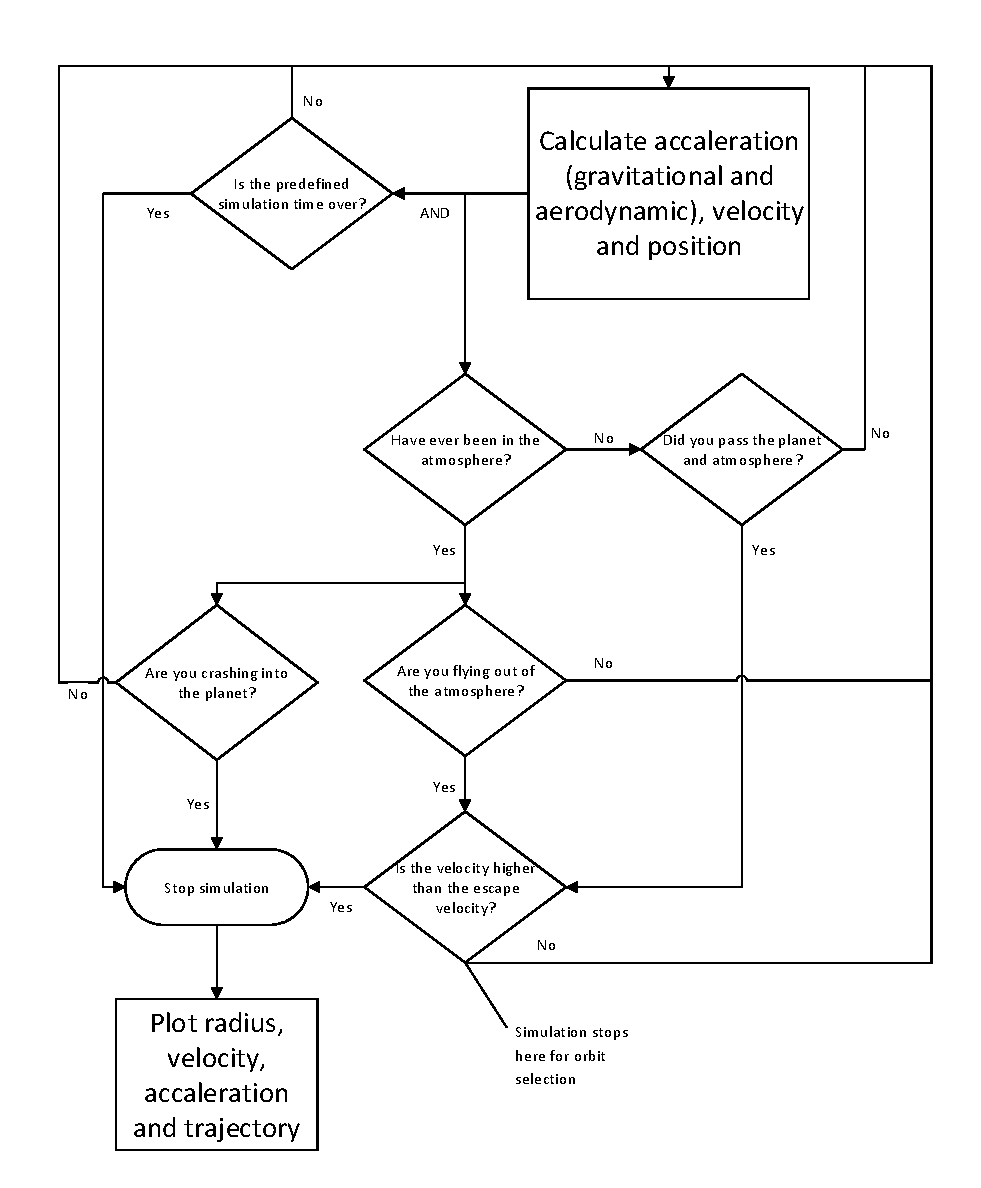
\includegraphics[width = 0.8\textwidth]{Figure/astro_tool.pdf}
\vspace{-5mm}
\caption{Flowchart of the decision making structure of the trajectory analysis program}
\label{fig:traj_flow}
\end{figure}

\subsection{Verification and validation}